\documentclass[12pt]{article}
\setcounter{secnumdepth}{0} % Remove numbering
\usepackage[a4paper, left=0.9in, right=0.9in, top=1.0in, bottom=1.0in]{geometry}
\usepackage{graphicx}   % Required for inserting images
\usepackage{tocloft}    % Include the tocloft package for customizing the TOC
\usepackage{titlesec}
\usepackage{caption}
\usepackage{float}
\usepackage[newfloat]{minted}

% Add a line after each section
\titleformat{\section}
  {\normalfont\Large\bfseries\centering}{\thesection}{1em}{}[{\titlerule[0.1pt]}]

% Add dots and borders in the table of contents
\renewcommand{\cftpartleader}{\cftdotfill{\cftdotsep}}      % Adds dots between part entries
\renewcommand{\cftpartfont}{\bfseries}                      % Part entries in bold
\renewcommand{\cftpartpagefont}{\normalfont}                % Page numbers in normal font

\renewcommand{\cftsecleader}{\cftdotfill{\cftdotsep}}       % Adds dots between section entries
\renewcommand{\cftsecfont}{\bfseries}                       % Section entries in bold
\renewcommand{\cftsecpagefont}{\normalfont}                 % Page numbers in normal font

\renewcommand{\cftsubsecleader}{\cftdotfill{\cftdotsep}}    % Adds dots between subsection entries
\renewcommand{\cftsubsecpagefont}{\normalfont}              % Page numbers in normal font

\setlength{\cftbeforepartskip}{0.5em}                       % Adjust the space before part entries
\setlength{\cftbeforesecskip}{0.3em}                        % Adjust the space before section entries
\setlength{\cftbeforesubsecskip}{0.1em}                     % Adjust the space before subsection entries

\renewcommand*\contentsname{}



\begin{document}

\thispagestyle{empty}   % Removes page number from the first page
\begin{center}
    \vspace*{\fill}     % Vertically center content

    \huge Colegiul National Bilingv

    \huge "George Cosbuc"

    \vspace{4cm}

    \textbf{\Huge The Impact of C, UNIX, and Pioneers Dennis Ritchie \& Ken Thompson}

    \vspace{10cm}

    \begin{minipage}[t]{0.5\textwidth}
        \Large \textbf{Elev:}
        \large Sorin-Andrei Tudose \\
        \Large \textbf{Clasa:}
        \Large $12R_2$
    \end{minipage}%
    \begin{minipage}[t]{0.5\textwidth}
        \raggedleft
        \Large \textbf{Profesor coordonator:} \\
        \large Kerestély Melinda Laura
    \end{minipage}

    \vspace*{\fill}     % Vertically center content
\end{center}


\newpage
\begin{center}
    \vspace*{\fill}     % Vertically center content
    \Huge\textbf{Table of Contents}
    \par\noindent\rule{\textwidth}{0.4pt}
    \small\tableofcontents
    \vspace*{\fill}     % Vertically center content
\end{center}

\newpage
\section{Synopsis}
What has always fascinated me is computer programming and software engineering.
After a few years of using a computer as a means of playing games I started wondering how those application run and their build process.
There were a few questions for which I really needed to find the answer, such as: How are games and other applications built?, How are different pieces of information displayed on the screen?,
How one can master the necessary skills to write a computer program?, etc. So I started doing research. Even thought, at that time, the documentation I was reading overwhelmed me,
I managed to understand that if one had the necessary knowledge, the possibilities in software engineering are endless. Since I wrote my first \verb|"Hello world"| in C\texttt{++}, when I was 15 years old,
I knew that hardware and software was the area I wanted to excel in. I find it truly magical how people can manipulate every pixel of a computer screen and display any desired content.\newline\newline
As a result, creating code and building applications, that help in solving different problems and enable us to be more effective is what I am keen on pursuing in my near future.
It is undoubtedly a complex field where mathematical and physics skills are required, but the excitement and passion for this field helps me overcome all challenges. \newline\newline
aving said that, I decided to write my Grade 12 Graduation Paper about \textbf{Dennis Ritchie} and \textbf{Ken Thompson} who revolutionized, in \textbf{1969} at \textbf{Bell Telephone Laboratories},
the way people used computers. Not only did they create the \underline{\textbf{UNIX}} operating system which is the root of many modern operating systems, but they also developed the \underline{\textbf{C}}
programming language. I, for one, am amazed of the things they created considering the fact that resources were not as broadly available as they are nowadays.
There were almost no applications designed for creating software and no internet that can assist with the process. In addition, they also had to write most of the code is Machine Language,
a low level programming language which takes a long time to master.\newline
\begin{center}
    Throughout this thesis we will go on a journey tracing the origins of computers.\newline
\end{center}

\section{Introduction}
These days most people own at least one modern computer for personal usage. As a result many do not know that the original design looked nothing like it does today.\newline\newline
First and foremost, there were no operating systems, programming languages, mice or keyboards. Moreover, there was no \textbf{physical storage} (\textit{solid-state drives} or \textit{hard disk drives}),
\textbf{RAM} memory (\textit{random access memory}) or \textbf{ROM} memory (\textit{read only memory}). \textbf{ENIAC} (\textit{Electronic Numerical Integrator and Computer}) (\textit{Figure 1}),
the very first computer designed at the University of Pennsylvania in 1945 to serve as a military tool to properly calculate the angle of elevation of a gun. This computer consumed around 150,000 watts
which is significantly higher than modern computers (200-500 watts).\newline\newline \textbf{So how did ENIAC work?}\newline\newline
Not only did it use several cables and switches, which were used to start, shut down and control the flow of data, but also plugboards, electrical switchboards into which electrical plugs are inserted to
create different temporary circuits, for transmitting instructions to the machine. As a result, for each task the computer needed manual calibration which meant rewiring the plugboards and adjusting the switches.
This “programming” method was not efficient in terms of flexibility and speed.

\begin{figure}[H]
    \centering
    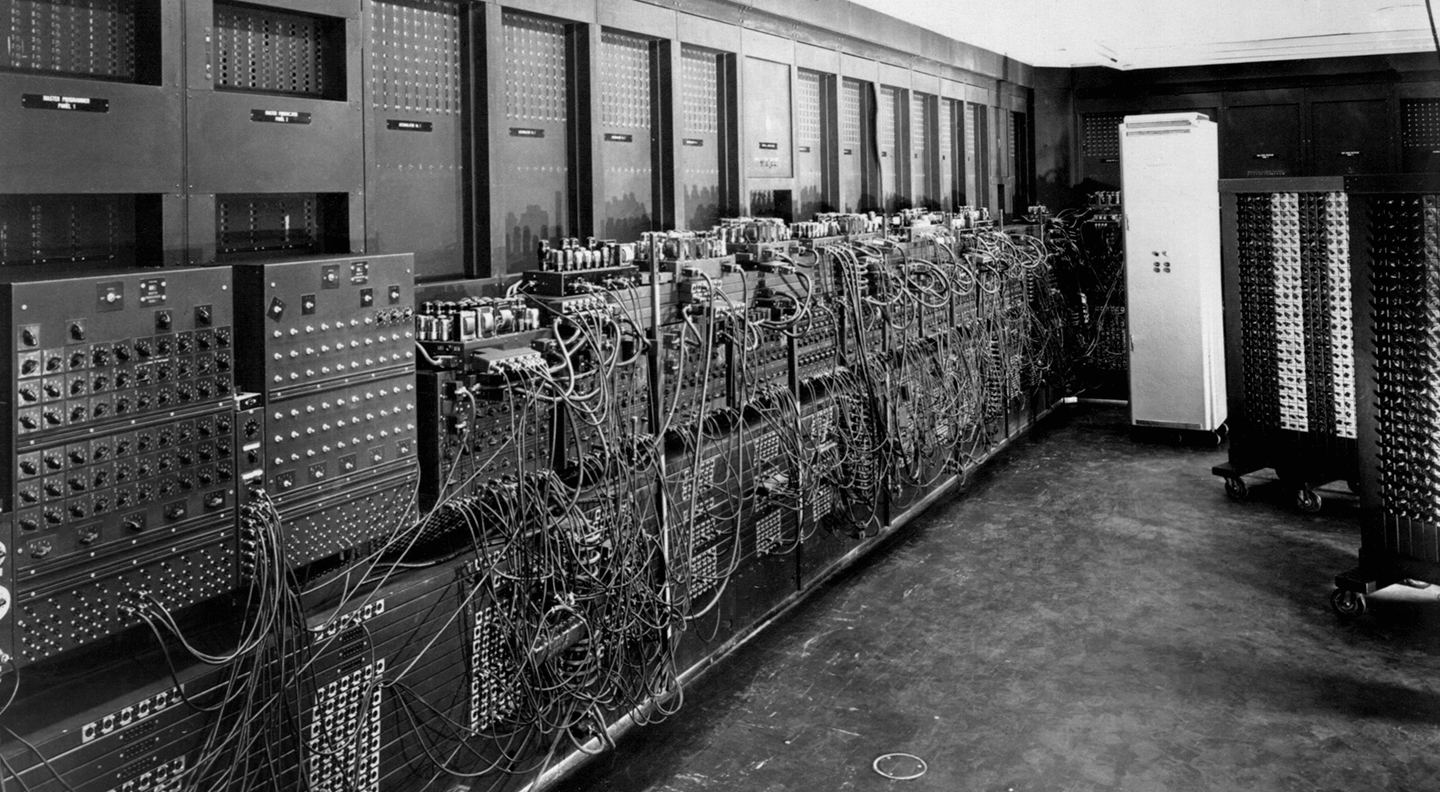
\includegraphics[width=10cm, height=5cm]{images/ENIAC.png}
    \caption{ENIAC}
\end{figure}

\begin{center}
    \footnotesize“Preparing ENIAC for a series of runs was an incredibly involved process. First, detailed instructions had to be written defining the problem and a procedure for solving it. These instructions were programmed by adjusting switches manually and inserting thousands of cables into as many as forty large plug boards. A team of five operators might work several days on the external wiring and many more days searching for errors and correcting them.”\textbf{ — Breakthrough to the Computer Age, Harry Wulforst, Charles Scribner’s \& Sons Pub., 1982}
\end{center}

\noindent After experimenting with ENIAC, people found different ways to make significant improvements:
\begin{itemize}
    \item (1949) \textbf{EDSAC} and \textbf{EDVAC} - Computers get memory as tubes with mercury
    \item (1949) \textbf{BINAC} - Programming languages were introduced (\textbf{William Schmitt} – Short Order Code)
    \item (1952) \textbf{IBM 701} - The first computer to use the assembler-style language (low-level programming language, used to directly communicate with the computer hardware) (\textit{Figure 2}) and a repository to store frequently used blocks of data.
          \begin{figure}[H]
              \centering
              \begin{minted}[
            linenos,        % Enable line numbers
            frame=lines,    % Set frame style
            framesep=2mm,   % Padding around frame
            baselinestretch=1.2, % Adjust line spacing
            fontsize=\footnotesize, % Adjust font size
            ]{text}
        *ASM     XOPTS(LEASM)
        DFHEISTG DSECT
        OUTAREA  DS    CL200                    DATA OUTPUT AREA
        *
        TESTLE   DFHEIENT CODEREG=R3
                 MVC OUTAREA(40),MSG1
                 MVC OUTAREA(4),EIBTRMID
                 EXEC CICS SEND TEXT FROM(OUTAREA) LENGTH(43) FREEKB ERASE
                 EXEC CICS RECEIVE
                 MVC OUTAREA(13),MSG2
                 EXEC CICS SEND TEXT FROM(OUTAREA) LENGTH(13) FREEKB ERASE
                 EXEC CICS RETURN
        *
        MSG1     DC     C'xxxx: ASM program invoked. ENTER TO END.'
        MSG2     DC     C'PROGRAM ENDED'
                 DFHREGS
        CODEREG  EQU    R3
                 END
        \end{minted}
              \caption{IBM Assembler Language (\textbf{ASM})}
          \end{figure}
    \item (1969) The \textbf{UNIX Time-Sharing} Operating System\newline\newline
          This year laid the foundation for modern computing. The UNIX Operating System, brought into perspective new technologies such as: \textbf{a hierarchical file system} (\textit{Figure 3}),
          \textbf{multiple levels of file access permission}, \textbf{input/output redirection}, and \textbf{pipes} (\textit{a temporary connection between two or more commands, programs or processes}).

          \begin{figure}[H]
              \centering
              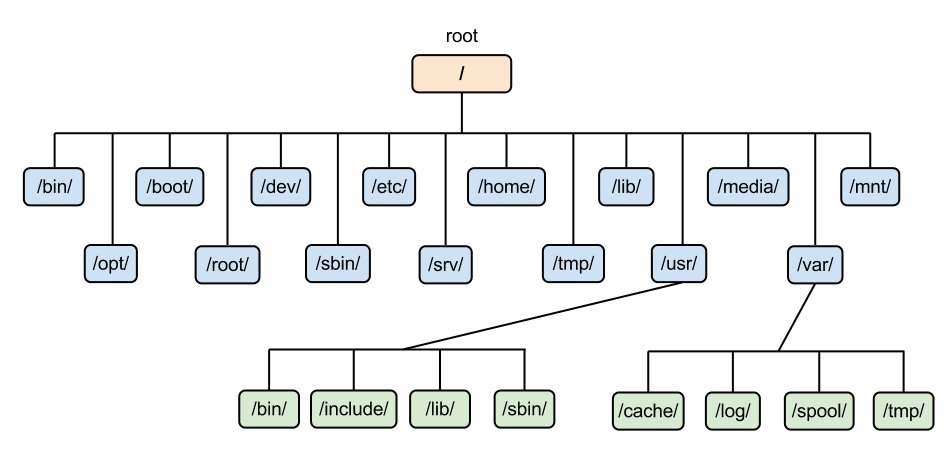
\includegraphics[width=14cm, height=7cm]{images/linux-filesystem.png}
              \caption{Hierarchical File System}
          \end{figure}

\end{itemize}

\newpage
\section{Dennis Ritchie \& Ken Thompson: C \& UNIX Pioneers}
During the late 1960s and early 1970s Ken Thompson and Dennis Ritchie worked as colleagues at the Bell Telephone Laboratories. Brian Kerninghan, who was part of the tehnical
staff at Bell Labs, describes Dennis Ritchie as \textit{"a really nice
    guy"}, who was really smart. Moreover, Kerninghan also aknowledges that Ritchie and Thompson had almost the same thinking process when creating computer alghorithms.
They wanted to create an operating system that supported multitasking, allowing users to run programs simultaneously. \newline\newline
Working together, they developed the \textbf{UNIX} Operating System using the high-level \textbf{C} programming language, designed by Ritchie.
The main issue this operating system solved was the compatibility between machines.
Computer software was specific to the hardware, therefore users would come find themselves using a machine with completely new command and operating procedures.
UNIX, being written using the \textbf{C} programming language, made it portable and adaptable. Moreover, UNIX also introduced pipes, which I briefly described in the introduction section.
This allowed different processes to communicate with each other and thus creating the possibility to run more complex tasks, more powerful workflows and automatisation. \newline\newline
One true passion that Ken Thompson had, was computer games. Taking in consideration the limtation of computer hardware and software at that time, game development was quite the challenge for software engineers.
Therefore, it took a lot of creativity and technical skills to successfully create a game. Not only did this hobby help him develop his alghoritmic thinking, but it also gave Thompson a deeper understanding of the early
computer systems.\newline\newline
\newpage
\section{Chapter 2: UNIX, the operating system revolution}

\newpage
\section{Chapter 3: The C programming language}
\subsection{C architecture: Unveiling the language's design}

\newpage
\subsection{Impact on programming languages \& software development}

\newpage
\subsection{The purpose behind C\texttt{++}}

\newpage
\section{Chapter 4 - The everlasting Legacy}
\subsection{Relevance of C and UNIX systems in today's technology}

\newpage
\subsection{The future of software development. 50 Years of C: Is it still worth learning?}

\newpage
\section{Conclusion}

\end{document}